\chapter{Introducción}
\label{chap:introduccion}

\section{Contextualización}
\textit{[Describir el entorno donde se identifica la necesidad del proyecto, indicando el sector, área de aplicación y situación actual. Incluir información relevante de la entidad receptora o del contexto donde se implementará la solución.]}


\section{Estado del Arte}
La Convención de la UNESCO para la Salvaguardia del Patrimonio Cultural Inmaterial reconoce como patrimonio a los usos, representaciones, expresiones, conocimientos y técnicas que las comunidades transmiten de generación en generación \cite{unesco2003convencion}. A partir de este marco, la revisión de la literatura se organizó en tres ejes: (i) aplicaciones digitales orientadas al patrimonio Kichwa y andino, (ii) gobernanza y soberanía de los datos indígenas, y (iii) aprendizaje móvil y georreferenciación aplicados a la difusión cultural.

\subsection{Soluciones digitales para el patrimonio Kichwa y andino}
El antecedente más directo es el trabajo de Quezada-Sarmiento \textit{et al.} \cite{quezada2026mobile}, quienes diseñaron un prototipo móvil educativo para el patrimonio cultural Saraguro y el aprendizaje introductorio del kichwa. La aplicación, desarrollada con la metodología ágil Mobile-D \cite{abrahamsson2004mobiled} sobre una arquitectura Android (MVVM) con servicios de Firebase, organiza contenidos de gastronomía, rituales y festividades, artesanías, medicina ancestral, relatos y lugares culturales en un mapa, además de expresiones básicas en kichwa con audio. La evaluación exploratoria con doce participantes reportó una buena claridad percibida y una alta valoración de los contenidos locales y georreferenciados. Sin embargo, los propios autores señalan limitaciones: ausencia de acceso sin conexión, soporte multilingüe reducido, falta de un protocolo estandarizado de usabilidad y ausencia de un módulo de administración y validación comunitaria de los contenidos.

En la misma línea, Quezada-Sarmiento \textit{et al.} \cite{quezada2026muleteering} abordan la arriería en Saraguro como patrimonio vivo y destacan el diálogo de saberes como estrategia de salvaguardia, mientras que Torres-Toukoumidis \textit{et al.} \cite{torres2022ancestral} analizan los rituales ancestrales de los Andes ecuatorianos como recurso de turismo comunitario. Ambos estudios confirman el valor de estas manifestaciones, aunque no proponen una plataforma tecnológica para su gestión.

\subsection{Gobernanza y soberanía de los datos indígenas}
La digitalización del patrimonio indígena plantea retos que van más allá de lo técnico. Christen \cite{christen2012information} cuestiona la idea de que toda la información deba ser de libre acceso y propone respetar los protocolos culturales de cada comunidad para determinar quién puede ver o compartir ciertos conocimientos. Kukutai y Taylor \cite{kukutai2016indigenous} y Hudson \textit{et al.} \cite{hudson2023indigenous} desarrollan el concepto de soberanía de los datos indígenas, según el cual los pueblos deben conservar el control sobre la información que se genera acerca de ellos. Linkola-Aikio \textit{et al.} \cite{linkola2025digital} complementan esta perspectiva con prácticas sostenibles para el patrimonio cultural indígena digital. Estos trabajos sustentan la necesidad de incorporar roles, permisos, consentimiento y validación comunitaria en la arquitectura propuesta.

\subsection{Aprendizaje móvil y georreferenciación}
Sarrab \textit{et al.} \cite{sarrab2012mobile} describen el aprendizaje móvil como una modalidad que amplía el acceso a recursos educativos en cualquier momento y lugar, lo que resulta pertinente para estudiantes y comunidades dispersas. Por su parte, Gretzel \textit{et al.} \cite{gretzel2015smart} muestran cómo las tecnologías basadas en la ubicación permiten interpretar territorios y recorridos, lo cual respalda el uso de mapas interactivos para vincular cada manifestación cultural con su espacio de origen.

\subsection{Análisis comparativo}
La Tabla~\ref{tab:estado_arte} resume los trabajos revisados, su aporte principal y su relación con el presente proyecto.

\begin{table}[htbp]
  \centering
  \caption{Comparación de los trabajos revisados en el estado del arte.}
  \label{tab:estado_arte}
  \small
  \begin{tabular}{|p{0.22\textwidth}|p{0.34\textwidth}|p{0.34\textwidth}|}
    \hline
    \textbf{Trabajo} & \textbf{Aporte principal} & \textbf{Limitación o brecha} \\
    \hline
    Quezada-Sarmiento \textit{et al.} \cite{quezada2026mobile} & App móvil con contenidos Saraguro, mapa y kichwa básico & Sin modo sin conexión, sin panel web de gestión ni validación comunitaria \\
    \hline
    Quezada-Sarmiento \textit{et al.} \cite{quezada2026muleteering} & Revitalización intercultural de la arriería como patrimonio vivo & No propone una solución tecnológica \\
    \hline
    Torres-Toukoumidis \textit{et al.} \cite{torres2022ancestral} & Rituales ancestrales andinos como turismo comunitario & Enfoque turístico, sin plataforma digital \\
    \hline
    Christen \cite{christen2012information}; Hudson \textit{et al.} \cite{hudson2023indigenous} & Protocolos culturales y soberanía de datos indígenas & Marco conceptual, sin implementación \\
    \hline
    Sarrab \textit{et al.} \cite{sarrab2012mobile}; Gretzel \textit{et al.} \cite{gretzel2015smart} & Aprendizaje móvil y tecnologías basadas en ubicación & No abordan el patrimonio Kichwa \\
    \hline
  \end{tabular}
\end{table}
\elaboradopor{Michael Jhosue Almeida Díaz}
\fuente{Elaboración propia}

En síntesis, las investigaciones revisadas validan la pertinencia de las tecnologías móviles y georreferenciadas para difundir el patrimonio Kichwa, pero ninguna integra en una misma solución una aplicación web de administración, una aplicación móvil con consulta sin conexión, un módulo de georreferenciación y mecanismos de validación comunitaria y control de acceso a contenidos sensibles. El presente proyecto toma como punto de partida el prototipo Saraguro \cite{quezada2026mobile} y busca cubrir esta brecha mediante la arquitectura multiplataforma propuesta.

\section{Planteamiento del Problema}
\textit{[Definir de forma clara y precisa el problema o brecha tecnológica identificada. Describir las causas que lo originan y los efectos que genera en el contexto analizado. No incluir la solución en esta sección.]}

\section{Justificación}
\textit{[Redactar un texto argumentativo que exponga la importancia del proyecto, su impacto técnico y operativo, la utilidad de la solución, los beneficiarios directos e indirectos y la factibilidad técnica y operativa de su implementación.]}

\section{Objetivos}
\subsection{Objetivo General}
Desarrollar una arquitectura multiplataforma web y móvil que permita gestionar, georreferenciar y difundir con fines educativos el patrimonio cultural inmaterial de los pueblos Kichwa de la Sierra Sur del Ecuador, mediante la integración de contenidos multimedia, recursos interactivos y mecanismos de participación comunitaria, con el propósito de contribuir a la preservación digital, valoración cultural y transmisión intergeneracional de sus saberes y tradiciones.

\subsection{Objetivos Específicos}
\begin{enumerate}
  \item Identificar y analizar los requerimientos funcionales, no funcionales, educativos y culturales de la plataforma, mediante la participación de docentes, investigadores, estudiantes y representantes de las comunidades Kichwa vinculadas con el proyecto Kallarimanta.
  \item Diseñar la arquitectura tecnológica, el modelo de datos y las interfaces de usuario de la solución web y móvil, considerando criterios de modularidad, escalabilidad, accesibilidad, seguridad, pertinencia cultural y conectividad limitada.
  \item Desarrollar una aplicación web administrativa que permita gestionar usuarios, comunidades, categorías, manifestaciones culturales, contenidos multimedia, ubicaciones geográficas y procesos de revisión y validación de la información.
  \item Implementar una aplicación móvil multiplataforma que facilite la consulta de contenidos culturales y educativos, la visualización de mapas interactivos, la búsqueda de información y el acceso limitado sin conexión a Internet.
  \item Integrar un módulo de georreferenciación para registrar y representar territorialmente comunidades, lugares y manifestaciones del patrimonio cultural inmaterial Kichwa de la Sierra Sur del Ecuador.
\end{enumerate}

\section{Alcance del Proyecto}
\textit{[Delimitar los límites del proyecto, especificando claramente los componentes, módulos o funcionalidades que se incluyen, así como aquellos que se excluyen.]}

\section{Fundamentación Teórica}
\textit{[Desarrollar los fundamentos teóricos, conceptos, modelos y tecnologías que sustentan el proyecto. Debe estar relacionado directamente con la solución propuesta y su implementación, aplicable a software, hardware o infraestructura.]}

\subsection{Ejemplo de Figura 1}
Como ejemplo de referencia dentro del texto: en la Figura~\ref{fig:ejemplo_1} se presenta un recurso visual demostrativo que guía el formato esperado para los gráficos del documento.

\begin{figure}[htbp]
  \centering
  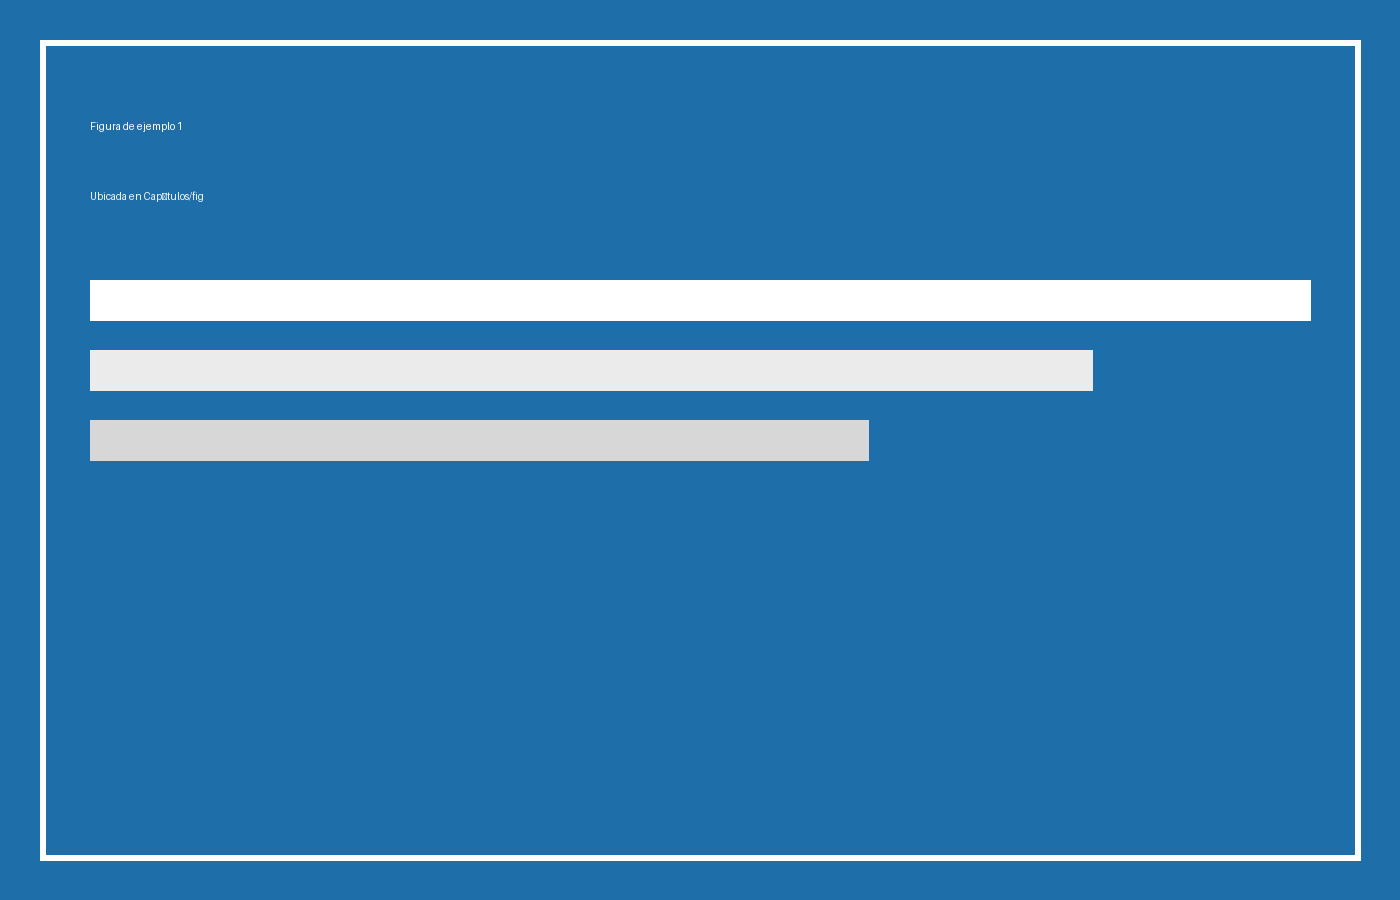
\includegraphics[width=0.80\textwidth]{Capítulos/fig/fig_ejemplo_1.png}
  \caption{Ejemplo de figura para guiar el formato de gráficos en el documento.}
  \label{fig:ejemplo_1}
\end{figure}
\elaboradopor{Estudiante}
\fuente{Elaboración propia}

\subsection{Ejemplo de Tabla 1}
Como ejemplo de referencia cruzada en párrafo: la Tabla~\ref{tab:ejemplo_1} resume indicadores base que luego pueden compararse con los resultados de implementación.

\begin{table}[htbp]
  \centering
  \caption{Ejemplo de tabla para registrar métricas iniciales del diagnóstico.}
  \label{tab:ejemplo_1}
  \begin{tabular}{|l|c|c|}
    \hline
    Indicador & Valor actual & Meta \\
    \hline
    Tiempo de respuesta (ms) & 850 & 400 \\
    \hline
    Disponibilidad (\%) & 96.2 & 99.0 \\
    \hline
    Incidencias mensuales & 14 & 6 \\
    \hline
  \end{tabular}
\end{table}
\elaboradopor{Estudiante}
\fuente{Datos de levantamiento inicial}
